\chapter{Methods}
\label{chapter:Methods}

% \section{Theorical Background}
The aim of this chapter is to define a basic workflow for the new detection approach
and provide the reader with relevant literature review. The workflow will be divided
in to different functional processes. The requirements (Input) and the outcome (Output)
of each process will be defined. Based on these requirements relevant theorical concepts
will be discussed. The processes directly related to the problem statement will be 
discussed in detail, and a suitable approach will be suggested. The reader should
note that this chapter will provide only the overview of the theorical concepts, 
implementation specific details will be covered in chapter \ref{chapter:Implementation} of the thesis.

To decide the best way to approach this problem, we need first knows our target for
the detection algorithm. In this case specifically, as we already mentioned, are fishes
within aquaculture enclosures. To understand in a better form our target, we begin
explaining the fish swimming mechanics, this will bring the necessary knowledge to define 
the strategy and possible constraint to our propose algorithm.

\subsection{Fish swimming mechanics}
A basic consideration for the design of algorithm to detect deformable object like fish are
their shape and pattern of movement. Studies have identified several types of locomotion that
fish use to generate thrust \citet{Hawkes2008,Colgate2004}. Most fish generate thrust by bending their
bodies into a backward-moving propulsive wave that extends to the caudal fin, a type of
swimming classified under body and/or caudal fin (BCF) locomotion. The propulsive wave traverses
the fish body in a direction opposite to the overall movement and at a speed greater than 
the overall swimming speed. There are four undulatory BCF locomation modes indetified by their
amplitude envelope of the propulsive wave: \textit{anguilliform, subcarangiform, 
carangiform and thunniform}. Despite these labels placed by biologists, two dimensions analyses
of the fish locomotion have shown that even fishes of very different body types show extremely similar 
patterns of body movement when viewed in a horizontal section during steady undulatory locomotion. 
Nevertheless, \textit{subcarangiform} swimming mode is the basis of the undulatory motion that present
the species which are farming in aquaculture project, like the Salmon and Trout.


\begin{figure}
\label{fig:fishlocomotion}
\centering     %%% not \center
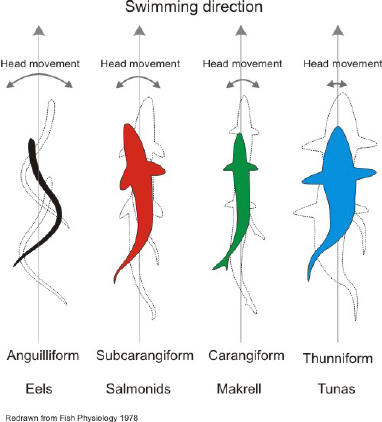
\includegraphics[width=70mm]{fishlocomotion}
\caption[]{This illustrate the classifications for fish locomotion, In our project
the most interested is the \textit{subcaringform}.\footnotemark{}}
\end{figure}
\footnotetext{Source: \url{http://esi.stanford.edu/exercise/exercise4.html}}

from the Figure \ref{fig:fishlocomotion}, what interest to us is the third class, the 
\textit{Carangiform} and \textit{subcaringform} locomotion model is describe as a movement
where only the posterior half of the body flexes with the passage of the contraction waves.


\begin{figure}
\begin{adjustwidth}{-1in}{-1in} 
\label{fig:fishswimming}
\centering     %%% not \center
\subfigure[]{\label{fig:a}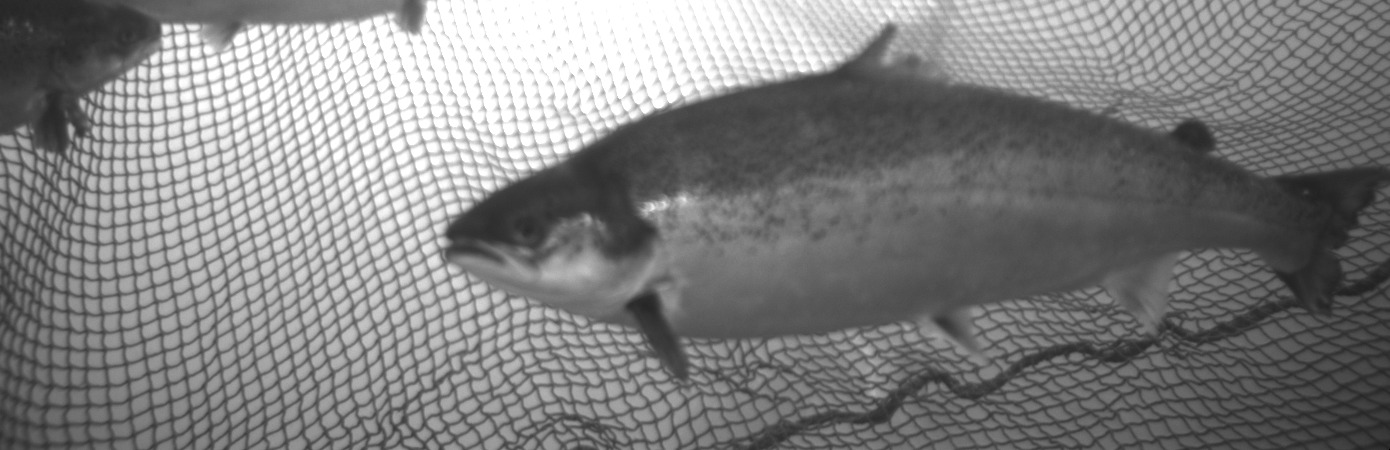
\includegraphics[width=70mm]{movement/data_st11_led0_0043}} \\
\subfigure[]{\label{fig:a}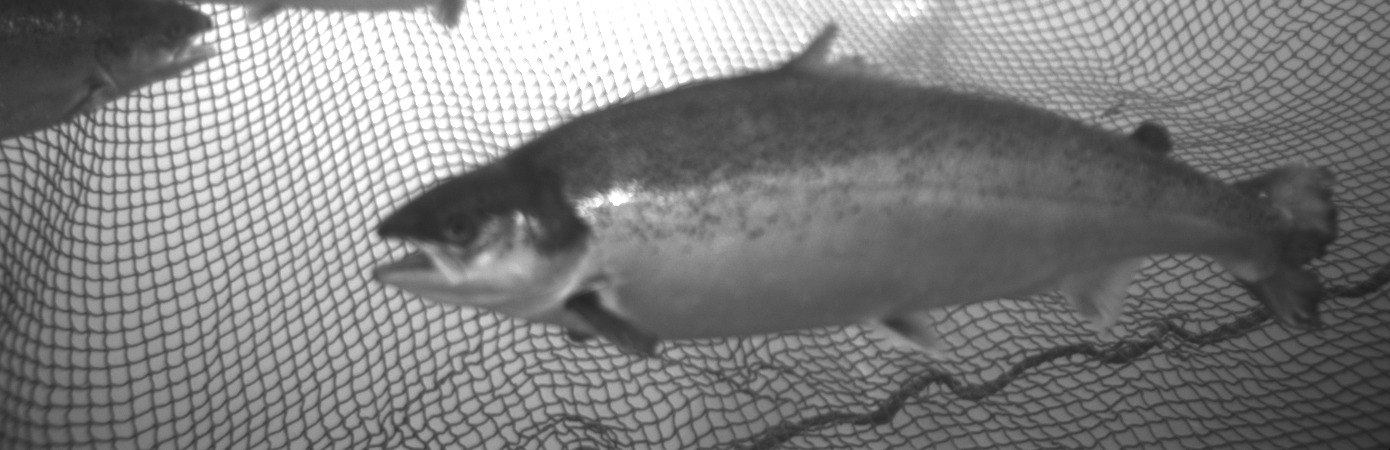
\includegraphics[width=70mm]{movement/data_st11_led0_0045}} \\
\subfigure[]{\label{fig:a}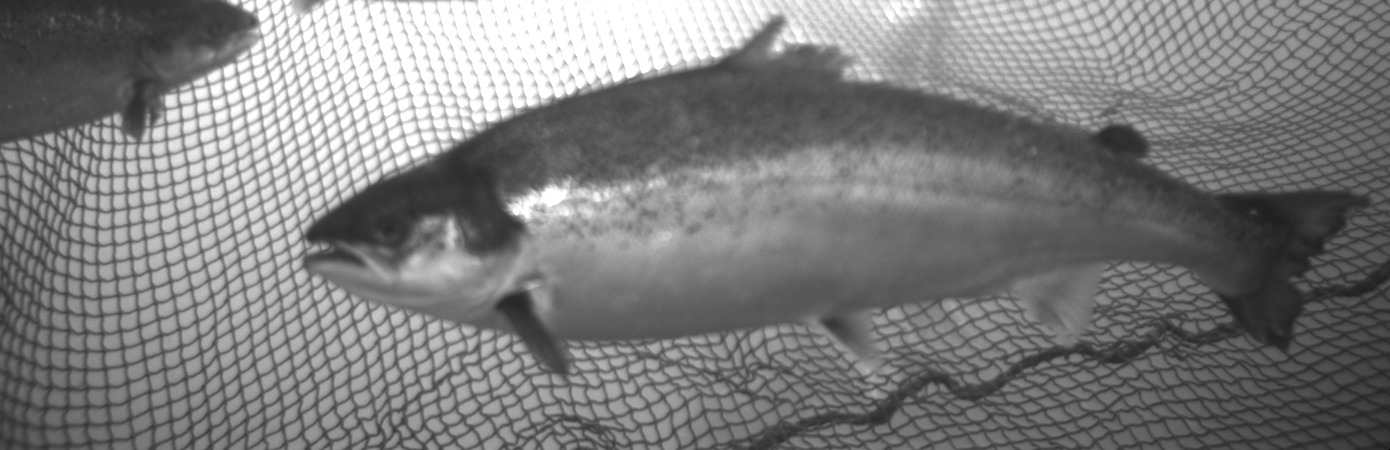
\includegraphics[width=70mm]{movement/data_st11_led0_0047}} \\
\subfigure[]{\label{fig:a}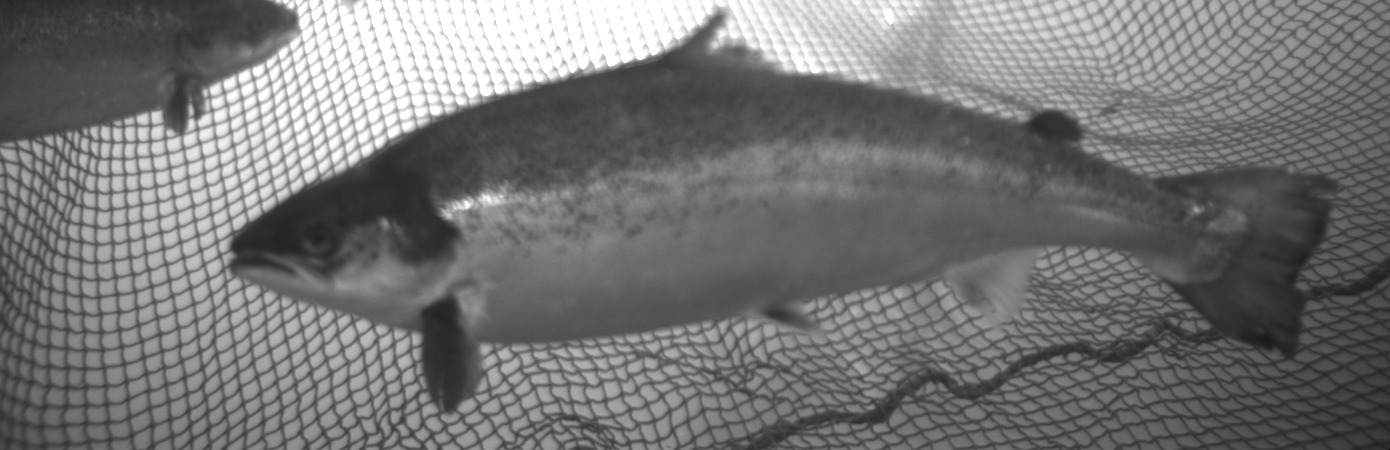
\includegraphics[width=70mm]{movement/data_st11_led0_0049}} \\
\subfigure[]{\label{fig:a}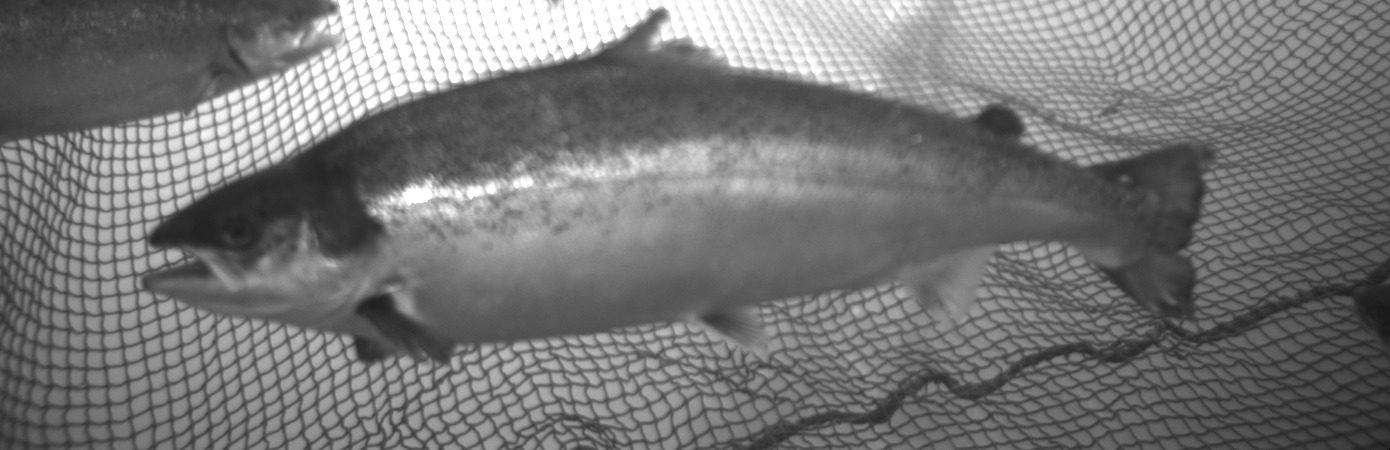
\includegraphics[width=70mm]{movement/data_st11_led0_0051}}
\caption{This illustrates a Salmon swimming in a aquaculture enclosure, here is possible to 
see that the tail present most part of the deformation in the fish body}
\end{adjustwidth}
\end{figure}


as shown in Figure \ref{fig:fishswimming}, most part of the deformation present in the fish
happen in the tail, and trough the backbone fish axis.
After review the physiological fish model, it is possible to infer that our algorithm
should model the fish, basically as a two part model, considering as a head-tail model.
The next section will introduce our propose approach.

\section{Notation and Symbols}
This section introduces the common mathematical notations and symbols used in this 
chapter.
Normal formatting such as $a$ and $A$ are used to indicate integers or real numbers 
while letters in scripts such $\mathcal{A}$ are reserved for sets. In addition, 
we use the symbols $\mathbb{R}$ for real numbers.
For 3D vectors, we use the uppercase bold letters $\mathbf{A}$ while for 2D vectors, 
we use the lowercase bold letters $\mathbf{a}$. If the vector if homogeneous, it will
be explicitly define; otherwise, the vector is assumed to be inhomogeneous. A vector
from point $A$ to $B$ is presented as $\overrightarrow{AB}$. Furthermore, matrices use
monospace font such as $\mathtt{A}$. If the dimension are specified such as $\mathtt{A}$$_{mxn}$,
$m$ would indicate the number of rows while $n$ indicates the numbers of columns.
Regardings accents, a hat on a vector such as $\hat{a}$ or $\hat{A}$ indicates the normalized
unit vector which means that $\hat{a}=\frac{a}{\|a\|}$ or $\hat{A}=\frac{A}{\|A\|}$.
A tilde on a 3D vector indicates that the last coordinate is removed; thus, the vector 
$A=(x,y,z)^T$ have $\hat{A}=(x,y)^T$  which is the projection of $A$ in the $xy$-axis,
while the vector with homogeneous coordinate $B=(x,y,z,1)^T$ have $\hat{B}=(x,y,z)^T$ 
which is the inhomogeneous coordinate of $B$. Lastly, a dot on top of variable indicates
the converged value of the variable after an algorithm is performed. For instances,
after using mean shift on $a_i$, it converges to a value $\dot{a}_i$

\section{Theorical Background and Propose Workflow}
\label{sec:workflow}

\begin{figure}[ht]
\centering
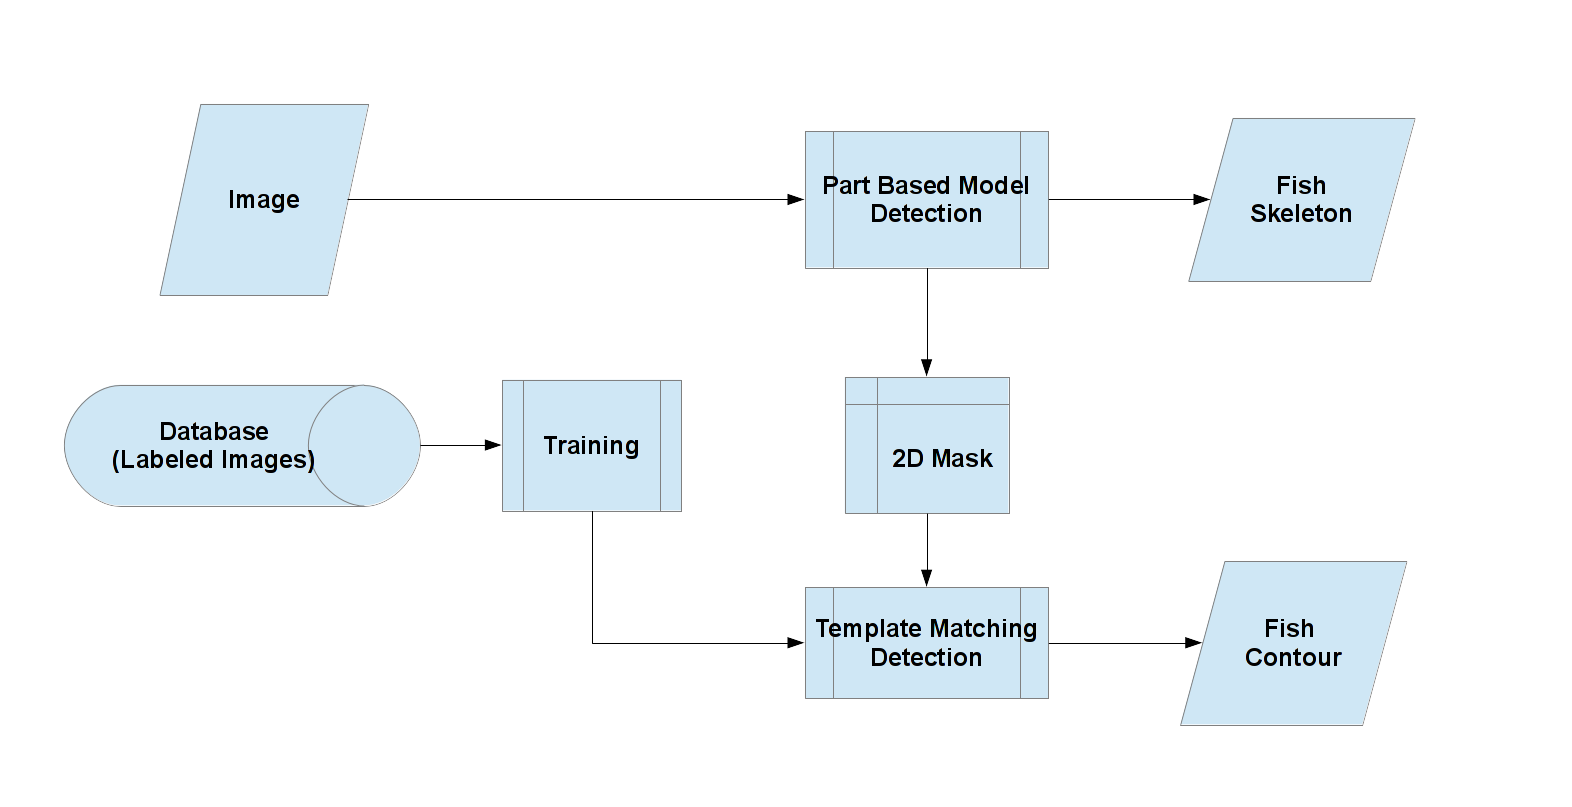
\includegraphics[scale=0.3]{flowchart_1}
\caption{A simplified workflow of the Detection process}
\label{fig:basicworkflow}
\end{figure}

Figure. \ref{fig:basicworkflow} shows the basic workflow of the detection process. The figure 
shows that once image is captured, it is supplied to the Part Based model detection 
process to extract 2D bounding boxes from the define part based fish model. Also from
this process can be extracted the skeleton of the fish, After 2D mask are generated, 
template detection matching process will take the 2D masked image and in those defined
areas will match the learned templates using the linemod algorithm propose in \citet{Hinterstoisser2012}. It is assumed that two detection process has been trained with the
proper labeled fish images in a offline procedure. A short introduction to the terms, processes and their functionalities is given below.

\begin{itemize}
\item \textit{Image}, this term refers to the two dimensional photographic image of the object
captured by the camera. It is given as a input for the detection workflow. The reader 
should note that the image provided to the workflow come from the underwater rig system
develop as part of the project.
which suggests that we are dealing with a deformable (articulated) object.
\item \textit{Database}, This term represents all the preprocessed information that 
is readily available to the detection workflow. This information includes details
regarding labeled data for training, trained model for Part Based detection process,
and trained model for template matching process.
\item \textit{2D Mask}, this term refer to the spatial filter, which in our problem
keep the spatial information result from the part based algorithm.
\item \textit{Part Based Model Detection}, this term refers to a broad class of 
detection algorithms used on images, in which various parts of the image are used 
separately in order to determine if and where an object of interest exists. 
Amongst these methods a very popular one is the constellation model which refers 
to those schemes which seek to detect a small number of features and their relative 
positions to then determine whether or not the object of interest is present. 
\item \textit{Template Matching Detection}, This term refers a broad class of algorithm
for finding small parts of an image which match a template image. this approach can be divide in
Feature-based and Template-based.
\item \textit{Training - Supervised Learning}, This term refers to the machine learning task
of inferring a function from labeled training data. The training data consist of a set of samples, 
where each sample is a pair of a input object and a desired output value.
\item \textit{Fish skeleton}, Correspond to simplified representation of the fish, as a set
of stick joining specific features in the body.
\item \textit{Fish Contour}, correspond to a curve along the fish silhouette
\end{itemize}

\subsection{Part Based model Detection}
\todo{redo the text to implement the problem}
In this section will be discuss the method used to achieve the first task define in \ref{sec:workflow},
analysing our target object, the fish, which can be model like a deformable object 
with one main deformation axis as show in the Figure \ref{fig:fishlocomotion}, at the beginning
of this chapter, the one define by the backbone, Most fish move by alternately contracting paired
sets of muscles on either side of the backbone. These contractions form S-shaped curves that move down the body.

\begin{figure}[ht]
\centering
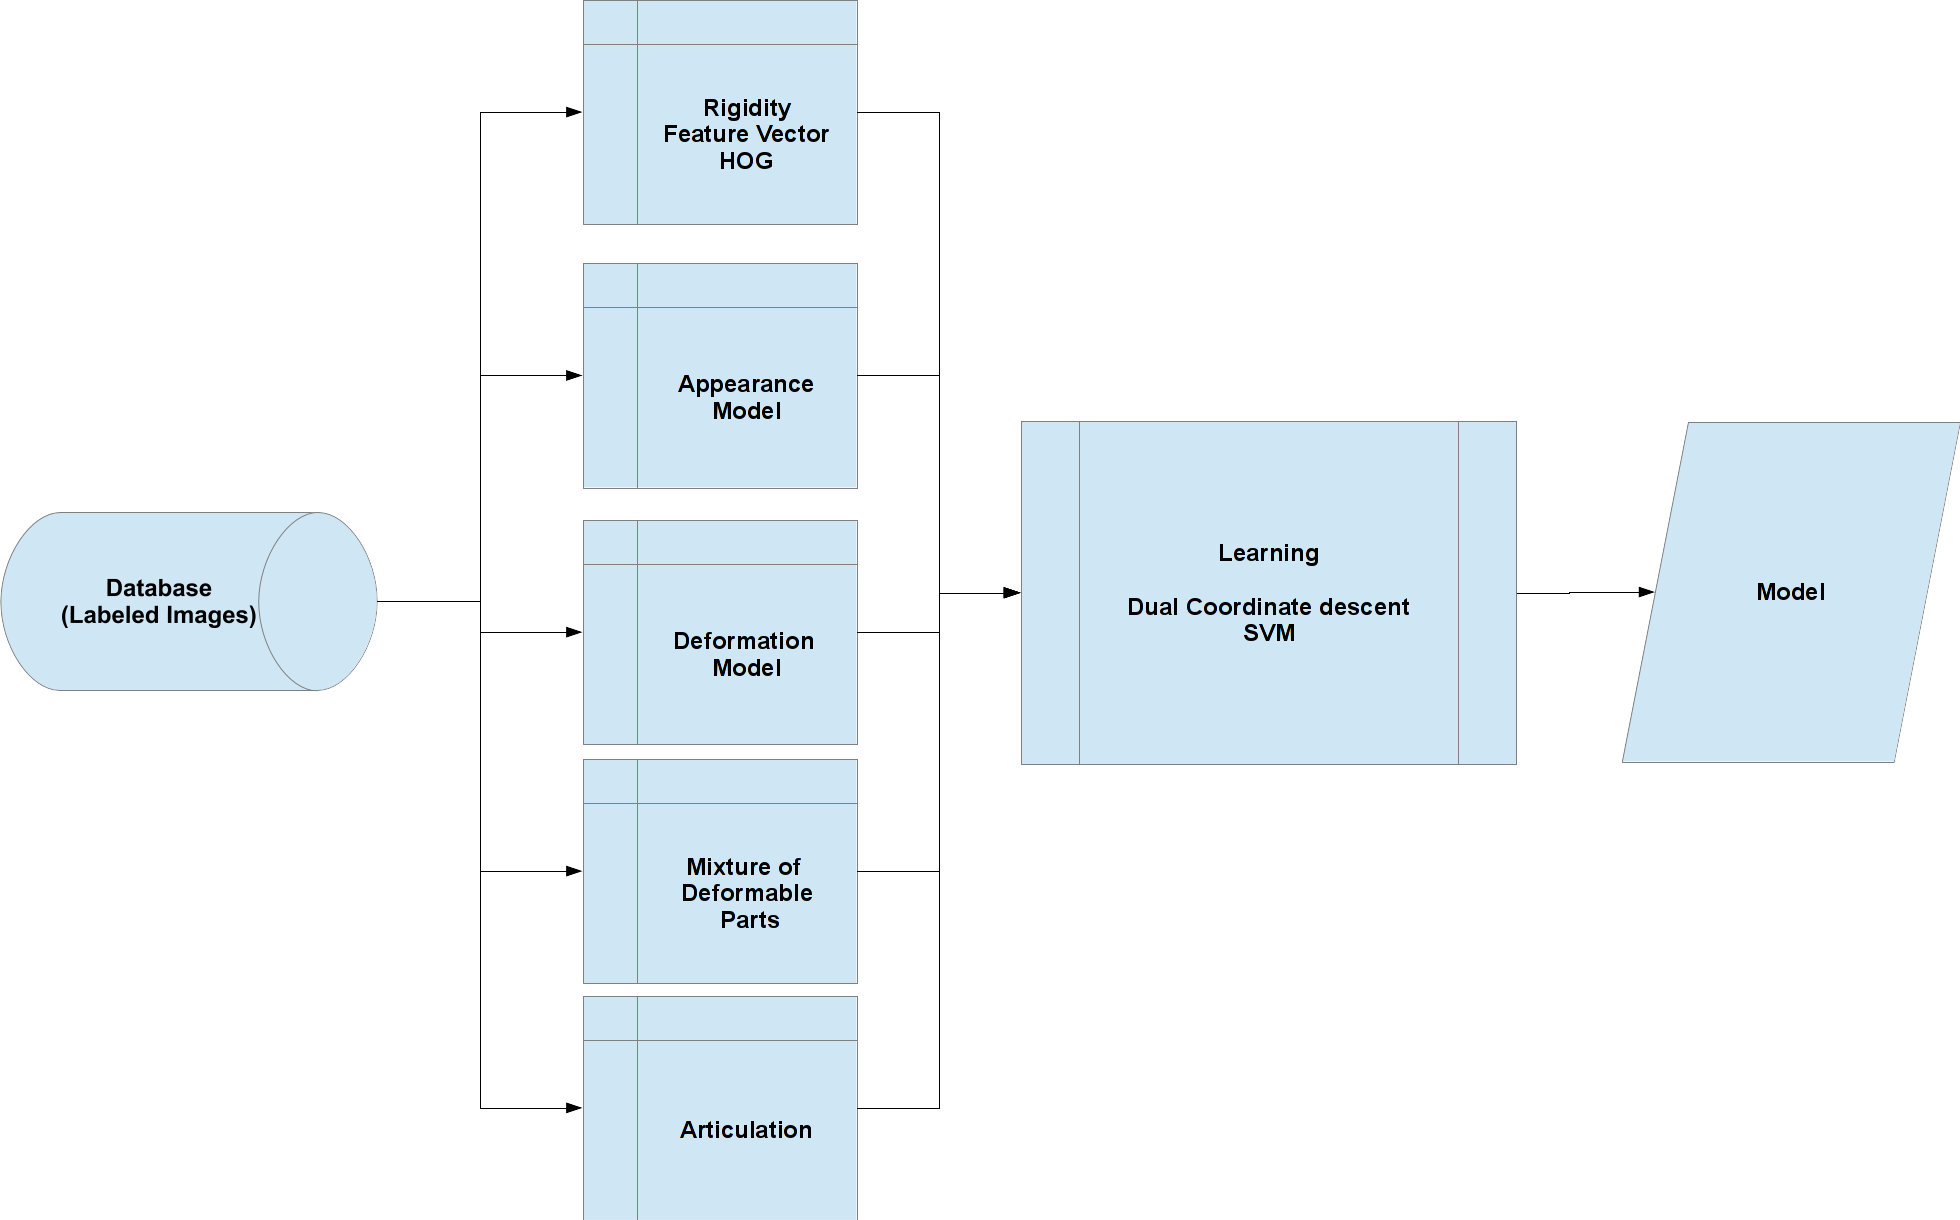
\includegraphics[width=160mm]{partbased/partbased02}
\caption{Simplified representation of Part based model detection - Mixtures of parts}
\label{fig:partbesed02}
\end{figure}

The pictorial structure framework arise as a feasible approach, which decomposes the appearance
of the objects into local part templates, together with geometric constraints on pairs of parts, 
often visualized as a spring. when parts are parametrized by pixel location and orientation, 
the resulting structure can model articulation. This has been the dominant approach for human
pose estimation. For our problem comparing with Full-body pose estimation where many degrees 
of freedom has to be estimated, The fish is a simplification due to the movement constraints,
and also the absence of big limbs which are replace by small fins, those fins not vary 
greatly in appearance in compare with human limbs. in the broad class of part based 
detection algorithm, the one propose by \citet{Ramanan2012} arise as the state of 
the arts, and is the one selected to be applied in
our problem.



\begin{figure}[ht]
\centering
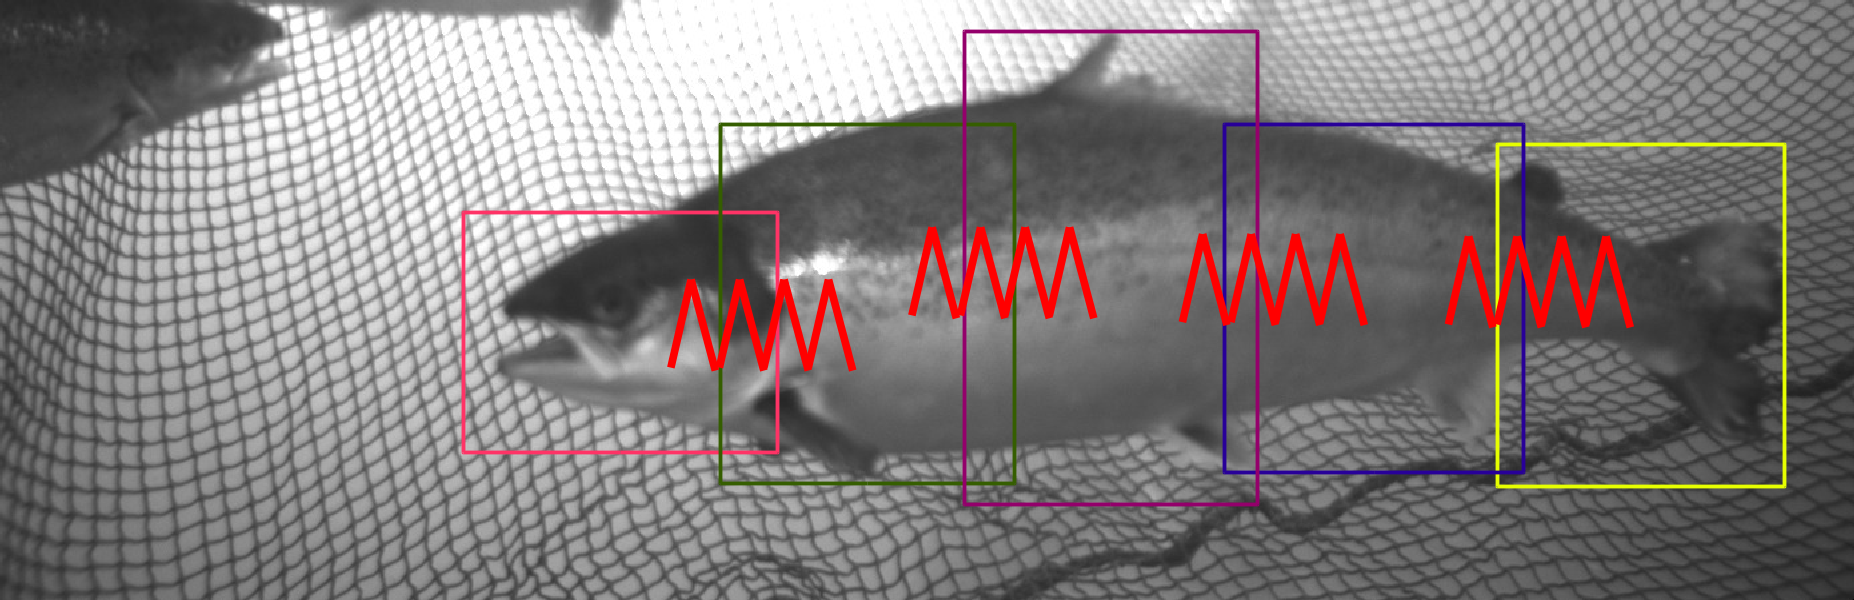
\includegraphics[width=80mm]{partbased/partbased01}
\caption{The flexible mixture-of-parts model approximate small warps by translating patches connected with spring.
Hence, this model captures the dependence of local part appearance on geometry.}
\label{fig:partbesed01}
\end{figure}

\subsubsection{Model}
Let us write $I$ for a image, $l_i = (x,y)$ for the pixel location of part $i$ and $t_i$ 
for the mixture component of part $i$. We write $i$ $\in$  $\{1\dotsc K\}$, $l_i \in \{1\dotsc L\}$ 
and $t_i \in \{1\dotsc T\}$. we call $t_i$ the ``type" of part $i$.
\todo{adapt example} Our motivating examples of types include orientations of parts 
(e.g., a vertical versus horizontally oriented hand), but types may span out-of-plane
rotations (front-view head versus side-view head) or even semantic classes 
(an open versus side-view head) or even semantic classes (an open versus closed hand). 
For notational convenience, we define lack of subscript to indicate a set spanned by that subscript
(e,g,. $t=\{t1\dotsc t_K\}$. For simplicity, we define our model at a fixed scale; 
at test time we detect people of different sizes by searching over an image pyramid.

\textit{Co-occurrence model:} To score of a configuration of parts, we first 
define a compatibility function for part types that factors into a sum of local and pairwise scores:
\begin{equation}
S(t)=\sum_{i\in V} b_i^{t_i} + \sum_{ij\in E} b_{ij}^{t_i,t_j}
\end{equation}

The parameter $b_i^{t_i}$ favors particular type assignments for part $i$, while
the pairwise parameter $b_ij^{t_i,t_j}$ favors particular co-occurrences of part types.
For example, if part types correspond to orientations and part $i$ and $j$ are on the
same rigid limb, then  $b_ij^{t_i,t_j}$ would favor consistent orientation assignments.
Specifically,  $b_ij^{t_i,t_j}$ should be a large positive number for consistent
orientations $t_i$ and $t_j$, and a large negative number for inconsistent orientations
$t_i$ and $t_j$.

\textit{Rigidity:} we write $G = (V,E)$ for a (tree-structured) $K-node$ relational
graph whose edges specify which pairs of parts are constrained to have consistent
relations.Such a graph can still encode relations between distant parts through transitivity.
For example, our model can force a collection of parts to share the same orientation,
so long as the parts to share the same orientation, so long as the parts form a connected
$subtree$ of $G = (V,E)$. We use this property to model multiple parts on the torso.
Since co-occurrence parameters are learned, our model learns which collections of parts should be rigid.
We can now write the full score associated with a configuration of part types and positions:
\begin{equation}
\label{eq:rigidity}
S(t,l,t)=S(t) + \sum_{i\in V} \omega_i^{t_i} \cdot \phi(I,l_i) + \sum_{ij\in E} \omega_{ij}^{t_i,t_j} \cdot \psi(l_i - l_j)
\end{equation}

where $\phi(I,l_i)$ is a feature vector( e.g, HOG descriptor \citet{Dalal2005})
extracted from pixel location $l_i$ in image $I$. we write $\psi(l_i - l_j)=[dx\; dx^2\; dy\; dy^2]^T$, 
where $dx=x_i - x_j$ and $dy=y_i - y_j$, the relative location is defined
with respect to the pixel grid and not the orientation of part $i$ (as in classic 
articulated pictorial structures).

\textit{Appearance model:} The first sum in \ref{eq:rigidity} is an appearance model 
that computes the local score of placing a template $\omega_i^{t_i}$ for part $i$,
tuned for type $t_i$, at location $l_i$.

\textit{Deformation model:} The Second term can be interpreted as a \"switching\"
spring model that controls the relative placement of part $i$ and part $j$ by switching
between a collection of springs. Each spring is tailored for a particular pair of 
types $(t_i,t_j)$, and is parametrized by its rest location and rigidity, which are 
encoded by $\omega_{ij}^{t_i, t_j}$.Our switching spring model encodes the dependence
of local appearance on geometry, since different pairs of local mixtures are constrained
to use different springs. Together with the co-occurrence term, it specifies an
image-independent ``prior" over part locations and types.

\textit{Mixture of deformable parts: } from \citet{Felzenszwalb2010} define a mixture of models, where each model is a star-based pictorial structure. This can be achieved by restricting the
co-occurrence model to allow for only globally-consistent types:

\begin{equation}
b_{ij}^{t_i,t_j}=\left\{ 
  \begin{array}{l l}
	0 & \quad \text{if $t_i=t_j$}\\
    -\infty & \quad \text{Otherwise}
  \end{array} \right.
\end{equation}

\textit{Articulation: } the author also propose a simplified version of \ref{eq:rigidity}
with a reduced set of springs:

\begin{equation}
\omega_{ij}^{t_i,t_j}\,=\,\omega_{ij}^{t_i}
\end{equation}


\subsubsection{Inference}
Inference corresponds to maximizing $S(I,l,t)$ from \ref{eq:rigidity} over $l$ and $t$.
When the relational graph $G=(V,E)$ is a tree, this can be done efficiently with 
dynamic programming. To illustrate inference, let us re-write \ref{eq:rigidity} by
defining $z_i = (l_i,t_i)$ to denote both the discrete pixel location and discrete
mixture type of part $i$:

\begin{equation}
\begin{split}
S(I,z) = \sum_{i \in V} \phi_i(I,z_i) + \sum_{ij \in E} \psi_ij(z_i,z_j), \\
where \quad \phi_i(I,z_i) = \omega_i^{t_i} \cdot \phi(I,l_i) + b_i^{t_i} \\
\quad \quad \psi_{ij}(z_i,z_j)=\omega_{ij}^{t_i,t_j} \cdot \psi(l_i -l_j)+b_{ij}^{t_i,t_j}
\end{split}
\end{equation}

From this perspective, it is clear that our final model is a discrete, pairwise Markov
random field $(MRF)$. When $G=(V,E)$ is tree-structure, one can compute $max_z\, S(I,z)$ 
with dynamic programming.

To be precise, we iterate over all parts starting from the leaves and moving ``upstream"
to the root part. We define kids$(i)$ be the set of children of part $i$, which is
the empty set for leaf parts. We compute the message part $i$ passes to its parent $j$
by the following:

\begin{equation}
\label{eq:inference1}
score_i(z_i)=\phi_i(I,z_i) + \sum_{k\in kids(i)} m_k(z_i)
\end{equation}

\begin{equation}
\label{eq:inference2}
m_i(z_j)=\max\limits_{z_i}\left[score_i(z_i) + \psi_{ij}(z_i,z_j)\right]
\end{equation}

\ref{eq:inference1} computes the local score of part $i$, at all pixel locations $l_i$ 
and for all possible types $t_i$, by collecting messages from the children of $i$. 
\ref{eq:inference2} computes for every location and possible type of part $i$, the
best scoring location and type of its child part $i$. Once messages are passed to the 
root part $(i=1)$, $score_1(z_1)$ represents the best scoring configuration for each 
root position and type. One can use these root scores to generate multiple detections in
 image $I$ by thresholding them and applying non-maximum suppression $(NMS)$. by keeping 
 track of the $argmax$ indices, one can backtrack to find the location and type of each 
 part in each maximal configuration. To find multiple detections anchored at the same 
 root, one can use $N-best$ extensions of dynamic programming.
\textit{Computation:} The computationally taxing portion of dynamic programming is 
\ref{eq:inference2}. We rewrite this step in detail:

\begin{equation}
\label{eq:inference3}
m_i(t_i, l_j) = \max\limits_{t_i}\left[b_{ij}^{t_i,t_j}+ \max\limits_{l_i}\, score_i(t_i,l_i)+\omega_{ij}^{t_i,t_j} \cdot \psi(l_i,l_j)\right] 
\end{equation}

one has to loop over $LxT$ possible parent locations and types, and compute a max 
over $LxT$ possible child locations and types, making the computation $O(L^2T^2$ 
for each part. When $psi(l_i-l_j)$ is a quadratic function (as is the case for us), 
the inner maximization in \ref{eq:inference3} can be efficiently computed for each
combination of $t_i$ and $t_j$ in $O(L)$ with a max-convolution or distance transform
\citet{Felzenszwalb2005}. Since one has to perform $T^2$ distance transforms, message passing
reduces to $O(LT^2)$ per part.



 \subsubsection{Learning}
 We assume a supervised learning paradigm. Given labeled positive examples ${I_n, l_n,t_n}$ 
and negative examples ${I_n}$, we will define a structured prediction objective 
function similar. To do so, let us write $l_n = (l_n, t_n)$ and note that the scoring
function \ref{eq:rigidity} is linear in model parameters $\beta=(\omega,b)$, and so
can be written as $S(I,z)=\beta \cdot \Phi(I,z)$. We would learn a model of the form:
\begin{equation}
\label{eq:learning}
\begin{split}
arg \quad mim_{\omega , \xi_n \geq 0} \quad \frac{1}{2}\beta \cdot \beta + C\sum_n \xi_n \\
s.t. \forall\,n\,\in\,pos \quad \beta \cdot \Phi(I_n, z_n) \geq 1 - \xi_n \\
\forall n \in neg, \forall z \quad \beta \cdot \Phi(I_n,z) \leq -1 + \xi_n
\end{split}
\end{equation}

The above constraint states that positive examples should score better than 1 (the margin),
while negative examples, for all configurations of part positions and types, should
score less than -1. The objective function penalizes violations of these constraints
using slack variables $\xi_n$.

\textit{Dual coordinate descent: } The currently fastest solver for linear SVMs appears to be
liblinear, which is a dual coordinate descent method. A naive implementation of a dual SVM solver would 
require maintaining a $MxM$ kernel matrix, where $M$ is the total number of active constraints
(support vectors). The innovation of liblinear is the realization that one can implicitly
represent the kernel matrix for linear SVMs by maintaining the primal weight vector $\beta$,
which is typically \textit{much} smaller. In practice, dual coordinate descent methods are efficient
enough to reach near-optimal solutions in a simple pass through large datasets.

In practice, to apply this algorithm, We define parts to be located at joints, so these provide
part position labels $l$, but not part type labels $t$.
\todo{maybe connect to implementation}

\subsection{Template based Model}
This technique has played an important role in tracking-by-detection applications for
many years. It is usually better adapted to low textured objects than feature point approaches. 
Unfortunately, this increased robustness often comes at the cost of
increased computational load that makes direct template matching inappropriate 
for real -time applications. This is especially true as many templates must be 
used to cover the range of possible viewpoints. for our application due of physical 
constraint of the camera rig system and the design of the aquaculture infrastructure
the viewpoints to the tracking object (Fish) is always coming from the side.
\todo{camera rig pic and cage setup}
from this viewpoints the amount of template necessary to have a proper result is reduce, as we explain at the beginning of this chapter. 

Our approach is based on the recent and efficient template matching methods from
\citet{Hinterstoisser2011, Hinterstoisser2012} which, for our approach, consider only the images and their
gradients to detect objects, because we not count with 3D data information.
As such, they work even when the object is not textured 
enough to use feature point techniques, and learn new object virtually instantaneously.
we based our solution in this algorithm, because has demostrated a great perfomance
in presence of strong background clutter and due the prior knowledge of the object
can handle in a better way occlusions, as the ones shows in the fig \ref{fig:clutter}.


\begin{figure}[ht]
\centering
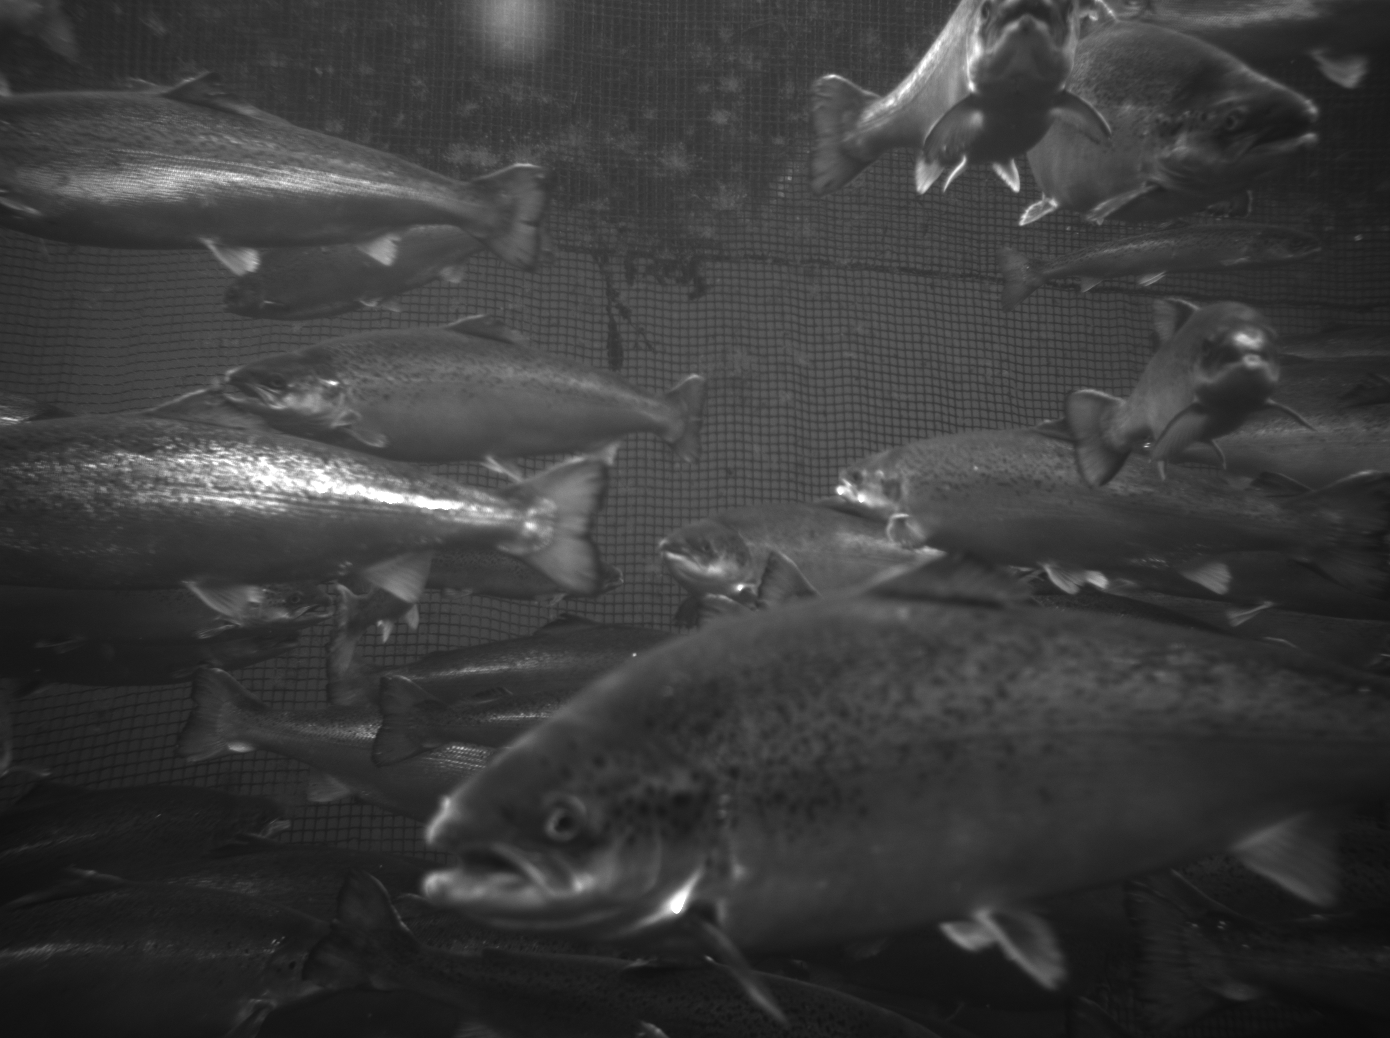
\includegraphics[width=80mm]{fish}
\caption{Fishes in aquaculture cage, heavily clutter background and occlusions}
\label{fig:clutter}
\end{figure}

Also the algorithm show being much faster for larger templates set. Instead of 
making the templates invariant to small deformations and translation by considering
dominant orientation only, the build a representation of the input images which has
similar invariance properties but consider all gradient orientations in local image
neighbourhood. Together with a novel similarity measure, this prevents problems due
to too strong gradients in the background. \todo{maybe a pic}.

This algorithm consider the modern CPU architecture through exploit heavy SSE parallelization, 
structuring the the images 
representation to  avoid ``memory cache misses" which slow down the computations.

\begin{figure}[ht]
\centering
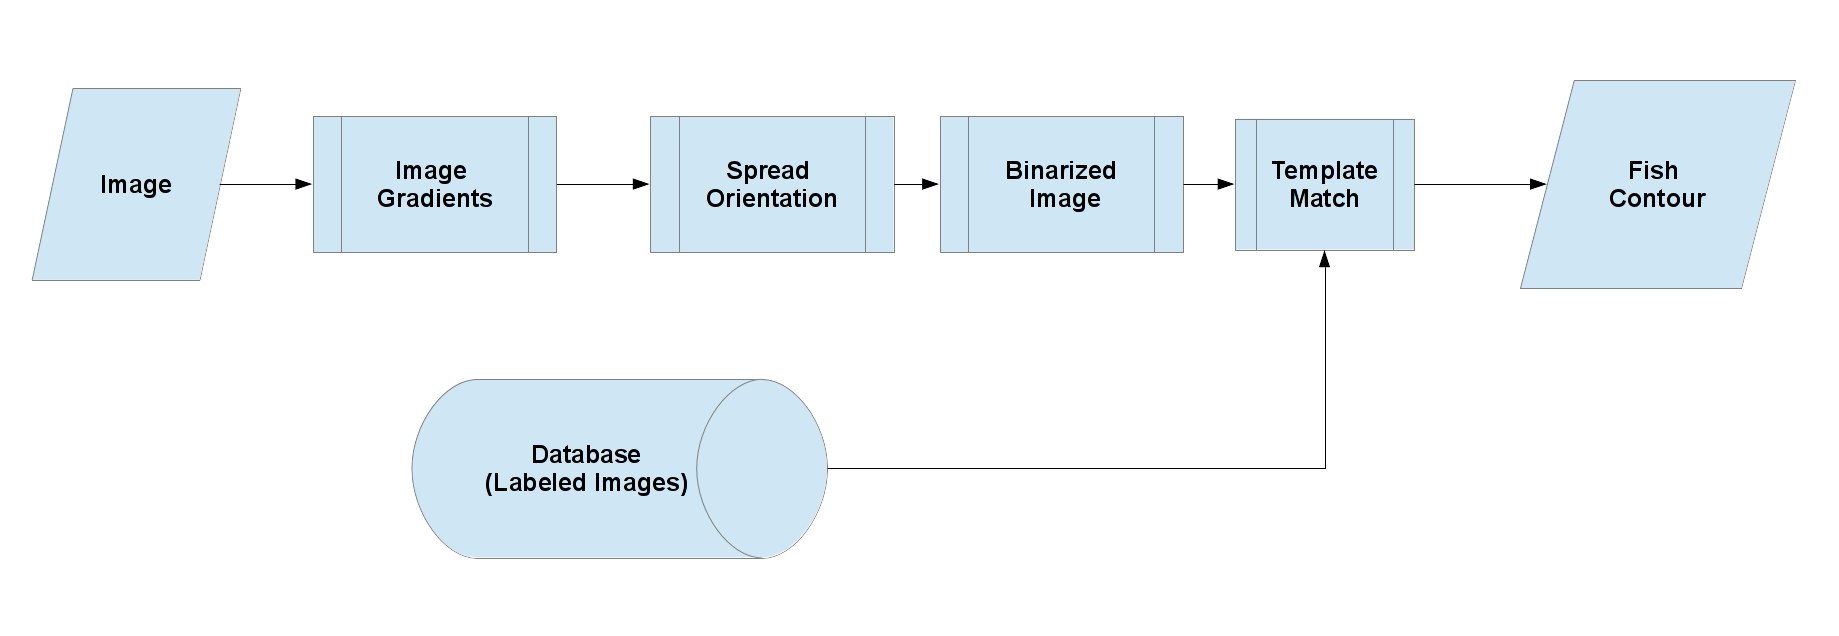
\includegraphics[width=140mm]{linemod/linemod}
\caption{Simplified flowchart of template based algorithm ``'LINEMOD" \citet{Hinterstoisser2011}}
\label{fig:clutter}
\end{figure}

\subsubsection{Model}
In this section, we describe the template representation and show how the representation 
of the input image can be use to parse the image to quickly find objects.
We will start by deriving the similarity measure, emphasizing the contribution of each 
aspect of it, \todo{check if we use this} it show how is implement the approach to
efficiently use modern processor architectures.

\subsubsection{Similarity Measure}
The unoptimized similarity measure can be seen as the measure defined by \citet{Steger2002} 
modified to be robust to small translations and deformations. 

\begin{equation}
\label{eq:similarity}
\varepsilon_{steger}(I, \tau, c) = \sum_{r \in P}\left| cos(ori(\Theta,r) - ori(I,c+r))\right|
\end{equation}

where $ori(\Theta,r)$ is the gradient orientation in radians at locations $r$ in a 
reference image $\Theta$ of an object to detect. Similarly, $ori(I,c+r)$ is the 
gradient orientation at $c$ shifted by $r$ in the input image $I$. We use a list,
denoted by $P$, to define the locations $r$ to be considered in $\Theta$. This way we
can deal with arbitrarily shaped objects efficiently. A template $\tau$ is therefore
defined as a pair $\tau=(\Theta,P)$.

Each template $tau$ is created by extracting a small set of its most discriminant
gradient orientations from the corresponding reference image as shown in Fig\todo{"fig"}
and by storing their locations. To extract the most discriminative gradients we consider
the strength of their norms. In this selection process, we also take the location
of the gradients into account to avoid an accumulation of gradient orientations in
one local area of the object while the rest of the object is not sufficiently described.

Considering only the gradient orientations and not their norms makes the measure
robust to contrast changes, and taking the absolute value of the cosine allows it
to correctly handle object occluding boundaries: It will not be affected if the object 
is over a dark background, or a bright background.

The similarity measure of Eq. \ref{eq:similarity} is very robust to background clutter,
but not to small shifts and deformations \todo{check}. A common solution is to first
quantize the orientations and to use local histograms like in SIFT \citet{Lowe2004} 
or HOG \citet{Dalal2005}. However this can be unstable when strong gradients appear 
in the background.

To overcome this issues, \citet{Hinterstoisser2011} introduce a similarity measure
that, for each gradient orientation on the object, searches in a neighbourhood of
the associated gradient location for the most similar orientation in the input image.
This can be formalized as:


\begin{equation}
\label{eq:newsimilarity}
\varepsilon(I, \tau, c) = \sum_{r \in P}\left( \max\limits_{t \in R(c+r)}\left|cos(ori(\Theta,r) - ori(I,t))\right|\right)
\end{equation}

where $R(c+r)=[c+r-\frac{T}{2}, c+r+\frac{T}{2}]\,X\,[c+r-\frac{T}{2}, c+r+\frac{T}{2}]$
defines the neighborhood of size $T$ centered on location $c+r$ in the input image.
Thus, for each gradient it is align the local neighborhood exactly to the associated 
location whereas in DOT, the gradient orientation is adjusted only to some regular grid. 
We show below how to compute this measure efficiently.

\subsubsection{Computing the Gradient Orientations}
Before to continue with the background, we shortly discuss why we use gradient orientations 
and how we extract them easily.
The chose to consider image gradients because they proved to be more discriminant than
other forms of representations, and are robust to illumination change and noise. Additionally,
 image gradients are often the only reliable image cue when it comes to 
texture-less objects. Considering only the orientation of the gradients and not their
norms makes the measure robust to contrast changes, and taking the absolute value of
cosine between them allows it to correctly handle object occluding boundaries: it will 
not be affected if the object is over a dark background or a bright background.
To increase robustness, this algorithm compute the orientation of the gradients on
each color channel of our input image separately and for each image location use the 
gradient orientation of the channel whose magnitude is largest. Given a RGB color image $I$, 
We compute the gradient orientation map $I_g$ at location $x$ with
\begin{equation}
I_g(x)=ori(\hat{C}(x))
\end{equation}

where

\begin{equation}
\hat{C}(x)=\arg \, \max\limits_{C \in {R,G,B}}\left\|\frac{\partial C}{\partial x}\right\|
\end{equation}

and $R,G,B$ are the RGB channels of the corresponding color image.

In order to quatize the gradient orientation map, the gradient direction is omit,
consider only the gradient orientation and divide the orientation space into $n_0$
equal spacing as shown in Fig. 3\todo{imagesss}. To make the quantization robust to 
noise, we assign to each location the gradient whose quantized orientation occurs most often in a $3 x 3$
neigbourhood. We also keep only the gradients whose norms are larger than a small
threshold.

\begin{figure}[ht]
\centering
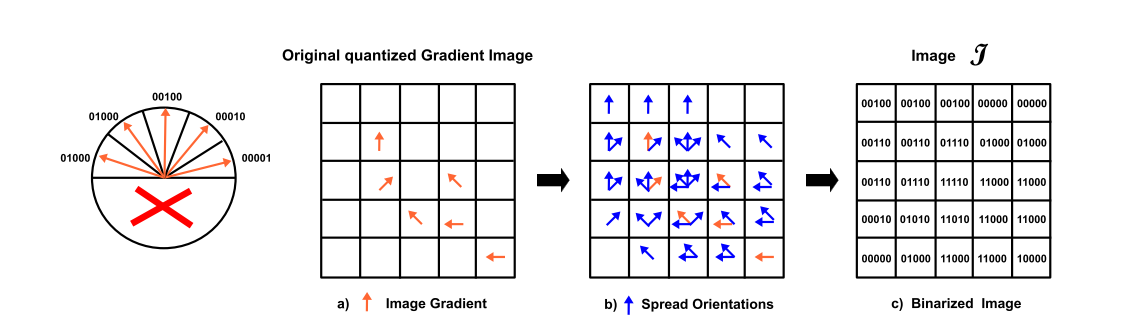
\includegraphics[width=140mm]{linemod/quantized}
\caption{Spreading the gradient orientations. Left: The gradient orientations and their binary code. We do not consider the direction of the gradients. a) The gradient orientations in the input image, shown in orange, are first extracted and quantized. b) Then, the locations around each orientation are also labeled with this orientation, as shown by the blue
arrows. This allows our similarity measure to be robust to small translations and deformations. c) J is an efficient representation of the orientations after this operation, and can be computed very quickly.}
\label{fig:clutter}
\end{figure}

\section{Propose Workflow}
After review the tools necessaries to acchieve our goal, 

% \IncMargin{1em}
\begin{adjustwidth}{-1in}{-1in} 
\begin{algorithm}
\label{algorithm:propose}
\SetKwData{Left}{left}\SetKwData{This}{this}\SetKwData{Up}{up}
\SetKwFunction{Union}{Union}\SetKwFunction{FindCompress}{FindCompress}
\SetKwInOut{Input}{input}\SetKwInOut{Output}{output}
\Input{A new Image $Im$ of the fishes}
\Input{Trained detector $Td_{pbmFish}$ Part Based model}
\Input{Trained detector $Td_{tmHead}$ Template matching for Head}
\Input{Trained detector $Td_{tmTail}$ Template matching for Tail}
\Output{Fish contour}
\BlankLine
\emph{	}\;
fishCandidates$\leftarrow$ getCanditeFromPartBasedModel($Im$, $Td_{pbmFish}$)\;
\ForEach{fishCandidate in fishCandidates}{
	\emph{Go through all fish candidates and apply template matching}\;
	headContours $\leftarrow$ contourbyLinemod($I_m$, $Td_{tmHead}$, fishCanditate.HeadBoundingBox)\;
	tailContours $\leftarrow$ contourbyLinemod($I_m$, $Td_{tmTail}$, fishCanditate.TailBoundingBox)\;
	\ForEach{headContour in headContours}{
		\emph{Go through all head contour and check if the are connected with the tail}\;
		\ForEach{tailContour in tailContours} {
			\If{tailContour connected with headContour}{
				Candidate $\leftarrow$ is Fish}
			\Else{
				continue}
		}
	}
}
\caption{Propose workflow for fish contour detection}\label{algo_disjdecomp}
\end{algorithm}
\end{adjustwidth}
% \DecMargin{1em}
